\documentclass[a4paper]{article}
\usepackage[frenchb]{babel}
\usepackage[utf8]{inputenc}
%\usepackage[T1]{fontenc}
%\usepackage{lmodern}
\usepackage{amsmath}
%\usepackage{tikz}
\usepackage{cite}
\usepackage{hyperref}
%\usepackage{fancyvrb}
%\usepackage{bm}
%\usepackage{pxfonts}
\usepackage{verbatim}
\usepackage{a4wide}
\usepackage{graphicx}

\hypersetup{
  backref=true, %permet d'ajouter des liens dans...
  pagebackref=true,%...les bibliographies
  hyperindex=true, %ajoute des liens dans les index
  colorlinks=true, %colorise les liens
  breaklinks=true, %permet le retour a la ligne dans les liens trop longs
  urlcolor=blue,  %couleur des hyperliens (blue pour la version web)
  linkcolor=blue, %couleur des liens internes (blue pour la version web)
  citecolor=blue, %couleur des citation (green pour la version web)
  bookmarks=true,  %cree des signets pour Acrobat
  bookmarksopen=true, %affiche completement les signets Acrobat
  %%%%%%%%%%%%%%%%% HYPER TITLE %%%%%%%%%%%%%%%%%%%%%%%%%%
  pdfsubject={Rapport} %document sous Acrobat.
}

% Alter some LaTeX defaults for better treatment of figures:
% See p.105 of "TeX Unbound" for suggested values.
% See pp. 199-200 of Lamport's "LaTeX" book for details.
% General parameters, for ALL pages:
\renewcommand{\topfraction}{0.9}  % max fraction of floats at top
\renewcommand{\bottomfraction}{0.8} % max fraction of floats at bottom
% Parameters for TEXT pages (not float pages):
\setcounter{topnumber}{2}
\setcounter{bottomnumber}{2}
\setcounter{totalnumber}{4}     % 2 may work better
\setcounter{dbltopnumber}{2}    % for 2-column pages
\renewcommand{\dbltopfraction}{0.9} % fit big float above 2-col. text
\renewcommand{\textfraction}{0.07}  % allow minimal text w. figs
% Parameters for FLOAT pages (not text pages):
\renewcommand{\floatpagefraction}{0.7}  % require fuller float pages
% N.B.: floatpagefraction MUST be less than topfraction !!
\renewcommand{\dblfloatpagefraction}{0.7} % require fuller float pages

% remember to use [htp] or [htpb] for placement


\newcommand{\FIXME}{\textcolor{red}{FIXME}}
%\newcommand{\TODO}[1]{(\textcolor{red}{TODO} #1)}
\newcommand{\TODO}[1]{}
\newcommand{\LANG}{{\sc Heptagon}}
\newcommand{\lucy}{{\sc Lucid Synchrone}}
\newcommand{\lustre}{{\sc Lustre}}
\newcommand{\scade}{{\sc Scade}}
\newcommand{\scadesix}{{\sc Scade~6}}
\newcommand{\minils}{{\sc MiniLS}}
\newcommand{\heptagon}{{\sc Heptagon}}
\newcommand{\obc}{{\sc Obc}}
\newcommand{\minivhdl}{{\sc MiniVHDL}}
\newcommand{\vhdl}{{\sc Vhdl}}

\newcommand{\bold}[1]{\textbf{#1}}
\newcommand{\p}[0]{\; \vert \;}
\newcommand{\rst}[1]{Rst(#1)}
\newcommand{\rstnd}[1]{RstNode(#1)}
% \newcommand{\rst}[1]{\llbracket #1 \rrbracket^{rst}}
\newcommand{\tvh}[2]{\llbracket #2 \rrbracket^{vhdl\ #1}}
\newcommand{\guardb}[1]{\llbracket #1 \rrbracket^{guard}}
\newcommand{\guard}[2]{\mbox{if } \guardb{#1} \mbox{ then } #2 \mbox{ else }
  \emptyset}
\newcommand{\mybox}[1]{\mbox{\tt{#1}}}
\newcommand{\bl}[0]{\hspace{0.45cm}}
\newcommand{\ind}[0]{\hspace{0.5cm}}
\newcommand{\Cons}[0]{\; \mathbf{::} \;}
\newcommand{\Coloneqq}[0]{::=}
\newcommand{\coloneqq}[0]{::=}
%% Syntaxe MiniLS

\newcommand{\Node}[4]{\mybox{node} \; f(#1) = #2 \; \mybox{with var} \
  #3 \; \mybox{in} \; #4}
\newcommand{\Op}[2]{\mybox{\bf{op}}(#1,\dots,#2)}
\newcommand{\Fby}[2]{#1 \, \mybox{fby}^{ck} \, #2}
\newcommand{\Pre}[1]{\mybox{pre}^{ck} \, #1}
\newcommand{\Every}[4]{#1^{ck}(#2,\dots,#3) \, \mybox{every} \, #4}
\newcommand{\App}[2]{#1^{ck}(#2)}
\newcommand{\If}[3]{\mybox{if} \; #1 \; \mybox{then} \; #2 \; \mybox{else} \; #3}
\newcommand{\When}[3]{#1 \; \mybox{when} \; #2(#3)}
\newcommand{\Merge}[5]{\mybox{merge} \; #1 \; (#2 \Rightarrow #3) \; \dots \; \
  (#4 \Rightarrow #5)}
\newcommand{\Merges}[5]{\mybox{merge} \; #1 \; (#2 \Rightarrow #3) \; \
  (#4 \Rightarrow #5)}
\newcommand{\Base}[0]{\mybox{base}}
\newcommand{\On}[3]{#1 \; \mybox{on} \; #2 (#3)}
\newcommand{\Map}[3]{\mathtt{map} \; #1\; n\; (#2,\dots,#3)}
\newcommand{\Fold}[3]{\mathtt{fold} \; #1\; n\; (#2,\dots,#3)}
\newcommand{\Mapfold}[3]{\mathtt{mapfold} \; #1\; n\; (#2,\dots,#3)}

%% Syntaxe VHDL

\newcommand{\Component}[6]{\mybox{component} \; #1 \; \mybox{port} \; #2 \; \
  \mybox{with} \; \mybox{sig} \; #3 \; \mybox{and} \; \mybox{var} \; #4 \; \\
  \mybox{and} \; \mybox{subcomponents} \; #5 \; \mybox{in} \; #6}

\newcommand{\Assign}[2]{#1 \Leftarrow #2}
\newcommand{\Affect}[2]{#1 \coloneqq #2}
\newcommand{\Case}[5]{\mybox{case} \; #1 \; \mybox{of} \; (#2 \Rightarrow #3) \
  \dots (#4 \Rightarrow #5)}

\title{Traduction SCADE/Lustre vers VHDL~\thanks{Rapport d'\'etude dans
    le cadre du projet GENCOD.}}  \author{Adrien Guatto et Marc Pouzet
  \\ LRI~\thanks{Marc Pouzet est maintenant professeur \`a l'Universit\'e
    Pierre et Marie Curie et rattach\'e \`a l'\'Ecole normale
    sup\'erieure. Adrien Guatto, \'etudiant de l'Universit\'e Pierre et
    Marie Curie, a effectu\'e son stage dans le cadre du projet.}}
\date{31 ao\^ut 2010}

\begin{document}

\maketitle

\section{Introduction}
Ce document pr\'esente le probl\`eme de la compilation d'un langage
synchrone tel que \scade{} vers un langage pour le mat\'eriel et les
circuits tel que \vhdl. Nous d\'ecrivons le probl\`eme pos\'e, les
principales solutions envisag\'ees et celle retenue par le LRI.

Ce travail s'est appuy\'e sur la r\'ealisation d'un prototype d'\'etude,
appel\'e \LANG{}. Il s'agit d'un compilateur produisant \`a la fois du
code s\'equentiel (ici, principalement C et Java) et du code \vhdl{} \`a
partir d'un programme synchrone. Le langage d'entr\'ee est un
sous-ensemble de \scadesix{} et en reprend les principales
constructions: \'equations data-flow, automates hi\'erarchiques et
tableaux. Son compilateur est organis\'e de mani\`ere similaire au
compilateur KCG de \scade{} d\'evelopp\'e par
Esterel-Technologies~\footnote{Pour \^etre complet, \LANG{} est aussi un
  sous-ensemble du langage \lucy~\cite{lucy:manual06} que nous avions
  d\'evelopp\'e pr\'ec\'edemment et qui a servi de cadre d'\'etude \`a la
  conception de \scadesix. Nous aurions donc pu r\'ealiser un prototype
  d'\'etude de la compilation vers \vhdl{} \`a partir de \lucy. Le langage
  \'etant plus riche (ordre sup\'erieur, inf\'erence de type, polymorphisme,
  etc.), cela n\'ecessitait de r\'esoudre des probl\`emes peu pertinents
  pour le projet GENCOD et nous \'eloignait de ce qui est r\'ealis\'e dans
  le compilateur KCG. D'o\`u le choix de consid\'erer un langage
  simplifi\'e, plus proche de \scadesix{} pour prototyper une \'eventuelle
\'evolution de KCG.}.  Le prototype \LANG{} a \'et\'e mis a la disposition des
partenaires du projet GENCOD.

\subsection{Compilation de SCADE/Lustre vers VHDL}

\begin{figure}[t]
\begin{center}
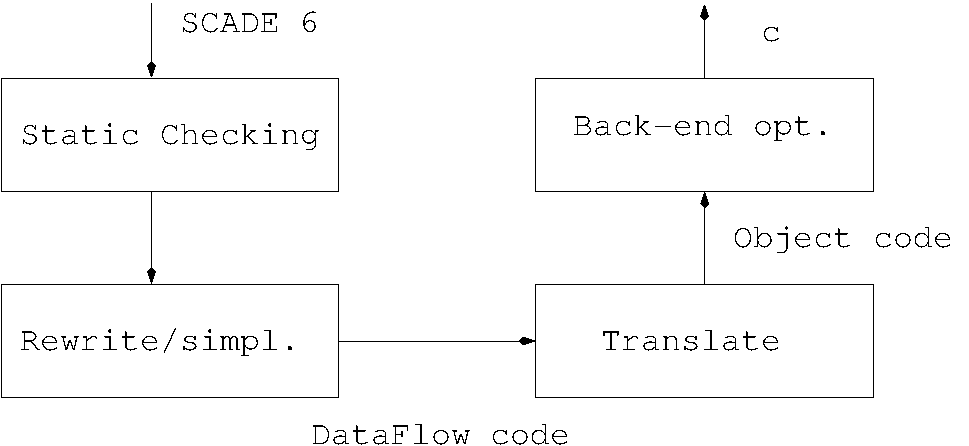
\includegraphics[height=4cm]{Fig/compil-scade}
\end{center}
\caption{Organisation g\'en\'erale du compilateur de SCADE~\label{organisation-scade}}
\end{figure}

Rappelons l'organisation g\'en\'erale du compilateur KCG
(Figure~\ref{organisation-scade}).  La compilation d'un programme se
d\'eroule en quatre grandes \'etapes: 1/ une phase d'analyse statique
(typage~\cite{lucy:emsoft03}, calcul d'horloges~\cite{lucy:emsoft04},
analyse de causalit\'e et analyse d'initialisation~\cite{lucy:sttt04});
2/ une phase comportant une succession de r\'e\'ecritures produisant \`a la
fin un code data-flow avec horloges; cette \'etape \'elimine les
principales structures de contr\^ole (automates, conditions
d'activations) en produisant des \'equations ``gard\'ees''; 3/ une phase
de compilation du code data-flow vers du code imp\'eratif s\'equentiel
(object code); chaque noeud \scade{} est repr\'esent\'e par une fonction
de transition; 4/ une phase d'optimisation appliqu\'ee au code
s\'equentiel (\'elimination des copies, propagation de constantes,
etc.). Au pr\'ealable \`a cette phase, les modules sont expans\'es et le
code polymorphe est sp\'ecialis\'e. Ces deux \'etapes pr\'eliminaires ne sont
pas d\'ecrites ici.

Au regard de cette organisation, il y a deux points d'entr\'ees naturels
pour produire du code \vhdl{}:
\begin{enumerate}
\item
\`a partir du code final g\'en\'er\'e par le compilateur (dans le cas de KCG, le
code C).
\item \`a partir du code interm\'ediaire data-flow avec horloges, apr\`es
  \'elimination des structures de contr\^ole (e.g., automates, conditions
  d'activation);
\end{enumerate}

Remarquons que le code interm\'ediaire data-flow est d\'ej\`a un point
d'entr\'ee pour les outils de v\'erification formelle utilis\'es dans le
compilateur KCG (tels que le plug-in de Prover Technology): la
v\'erification d'une propri\'et\'e (programm\'ee en \scade) est obtenue par
traduction pr\'ealable vers le format data-flow, format qui sert de
passerelle vers l'outil Prover.

\subsection{G\'en\'eration de VHDL \`a partir d'\'equations data-flow gard\'ees}
Les deux solutions d\'ecrites ci-dessus ont \'et\'e retenues dans le projet
GENCOD. La soci\'et\'e GeenSoft a r\'ealis\'e un compilateur \`a partir du code
C g\'en\'er\'e par KCG. Nous d\'ecrivons ici l'autre solution o\`u le code
\vhdl{} est produit directement \`a partir des \'equations data-flow. Pour cela,
nous d\'ecrivons formellement chacune des \'etapes de traduction, dans une
perspective d'int\'egration dans une cha\^{\i}ne de compilation certifi\'ee.

L'utilisation de Lustre pour la g\'en\'eration de mat\'eriel a \'et\'e envisag\'ee
tr\`es t\^ot (th\`ese de Fr\'ed\'eric Rocheteau~\cite{lustre:rocheteau91}). Signalons
\'egalement que \lustre{} est utilis\'e dans plusieurs enseignements de
mat\'eriel~\cite{lustre:amblard05}.

\subsubsection{Un mot sur la traduction de C vers VHDL}
L'int\'er\^et principal de produire du code \vhdl{} \`a partir du code C
g\'en\'er\'e par KCG est de ne pas toucher au compilateur existant, d\'ej\`a
qualifi\'e. \`A condition de qualifier le g\'en\'erateur de code C vers
\vhdl{} et de fournir les informations de retour au source
(tra\c{c}abilit\'e), on peut envisager de disposer d'une cha\^{\i}ne
compl\`ete qualifi\'ee. Discutons ici des points d\'elicats de cette solution.

La compilation de \scade{} est modulaire: un noeud \texttt{counter}
est traduit vers deux fonctions
C dont l'interface est sch\'ematiquement:

\begin{verbatim}
/* counter.c */
int counter_step(int counter_res, int counter_tick, counter_mem* self) { ... }

void counter_init(counter_mem* self)
  { self->counter_t1 = 0;
    self->counter_t2 = 0; }
\end{verbatim}
o\`u:
\begin{verbatim}
typedef struct { 
  int counter_t1; 
  int counter_t2; }
counter_mem;
\end{verbatim}
\texttt{counter\_step} est la fonction de transition qui prend
en entr\'ee un argument suppl\'ementaire repr\'esentant son \'etat interne. L'ex\'ecution
d'un pas produit une sortie et met \`a jour l'\'etat interne (par effet de bord).
La fonction \texttt{counter\_init} permet d'initialiser l'\'etat interne.

Le corps de ces deux fonctions est form\'e d'affectations de variables
locales o\`u de l'\'etat (ici \texttt{self->counter\_t1} et
\texttt{self-counter\_t2}) ainsi que de structures de contr\^ole
(conditionnelles, construction ``switch'' et boucles ``for'' o\`u
d'appel \`a d'autres fonctions de transition). La g\'en\'eration de code
\vhdl{} \`a partir du code s\'equentiel suit le sch\'ema suivant:

\begin{enumerate}
\item Une affectation de variable locale est traduite par une \'equation
  \vhdl{} sur une variable locale. E.g., \texttt{$x$ = $e$} est
  traduit en une instruction \vhdl{} \texttt{$x$ := $e$}.  Il faut
  cependant \^etre attentif \`a ce que \verb-x- ne g\'en\`ere pas de registre.
  Ce point est plus d\'elicat qu'il n'y parait, en particulier lors de
  la traduction d'un programme de la forme \texttt{if $cond$ \{ $x$ =
    $exp$; \}}. Il correspond \`a la d\'efinition d'un flot dont l'horloge
  est $cond$, c'est-\`a-dire que $x$ n'est d\'efinit qu'aux instant o\`u
  $cond$ est vrai. Parce que sa d\'efinition est partielle (la valeur de
  $x$ est ind\'efinie lorsque $cond$ est faux, sa traduction en \vhdl{}
  va conduire le synth\'etiseur \`a allouer un registre pour $x$, ce qui
  est \`a la fois inutile et inefficace.  Dans le cas o\`u le programme en
  entr\'ee n'a pas d'effets de bord, la s\'emantique de \scade{} garantit
  que ce programme est \'equivalent \`a l'affectation simple $x$ = $exp$. Par
  ailleurs, la s\'emantique de \scade{} garantit qu'aucun calcul de $x$ n'utilise
  la valeur de $x$ en dehors des instants o\`u $cond$ est vrai.
\item Une affectation de variable d'\'etat \texttt{self->$t$ =
    $exp$} doit \^etre traduite vers une instruction de la forme
  \texttt{$t$ <= $exp$}. Cette affectation doit cependant \^etre ex\'ecut\'ee
  conditionnellement. Il faut donc retrouver, dans le code C,
  la condition bool\'eenne d'activation de la mise \`a jour de
  l'\'etat \texttt{self->$t$}.
\item La compilation des it\'erateurs est \'egalement d\'elicate, en
  particulier lorsqu'ils sont appliqu\'es \`a des tableaux de bits. Une
  \'equation de la forme:
\begin{verbatim}
t1 = map not <<10>>(t0)
\end{verbatim}
o\`u \verb-t1- et \verb-t0- sont deux tableaux de taille 10 de valeurs
bool\'eennes. Le code imp\'eratif produit par le compilateur de \scade{} a
la forme suivante~\footnote{Nous donnons ici la sortie produite par le
  compilateur de \heptagon.}.
\begin{verbatim}
for (i = 0; i < 10; i++) {
  t1[i] = !t0[i]; }
\end{verbatim}
Or, le langage \vhdl{} dispose d'op\'erateurs agissant directement sur les
tableaux de bits (e.g., non logique, et logique). La bonne traduction
de la premi\`ere \'equation est donc:
\begin{verbatim}
t1 := not t0;
\end{verbatim}
La g\'en\'eration de ce code, si elle est triviale \`a partir du code format
data-flow --- il suffit de traduire specifiquement l'op\'eration
\verb-map not- --- est plus d\'elicate \`a partir du code imp\'eratif
traduit par KCG. Ceci d'autant plus que KCG applique plusieurs optimisations
sur les tableaux afin d'\'eliminer les copies successives et de fusionner
les boucles.
\end{enumerate}

Retenons ici qu'une information pr\'ecieuse pour la g\'en\'eration
de code \vhdl{} a \'et\'e perdue durant la compilation vers du code s\'equentiel et
doit donc \^etre reconstruite. Nous identifions trois autres
difficult\'es.
\begin{itemize}
\item La n\'ecessit\'e de certification demande d'instrumenter le
  compilateur KCG avec des informations donnant la tra\c{c}abilit\'e (lien
  entre les noms de variables produites et les noms dans le code
  source, en particulier).
\item Certaines optimisations pertinentes lorsque l'on g\'en\`ere du code
  s\'equentiel, peuvent ne pas \^etre utiles, voire p\'enalisantes, pour une
  compilation vers \vhdl{}. C'est le cas de l'optimisation des structures
  de contr\^ole ou de la compilation des boucles (cf. discussion
  ci-dessus, conduisant \`a g\'en\'erer trop de registres).
\item Il est n\'ecessaire de restreindre le p\'erim\`etre du compilateur C
  vers \vhdl{}: on ne r\'ealise pas un compilateur capable de traduire tout
  code C vers \vhdl{} mais plut\^ot un compilateur adapt\'e au code C produit
  par KCG et prenant en compte la technique de compilation
  sous-jacente. Comment alors d\'ecrire ce p\'erim\`etre ? Dans quel mesure
  le d\'eveloppement logiciel r\'ealis\'e s'appliquerait \`a un code C produit
  par un autre compilateur (e.g., issu de Simulink) ?
\end{itemize}

On peut enfin trouver peu naturel de passer par un langage
  interm\'ediaire s\'equentiel (ici C) pour compiler un langage parall\`ele
  tel que \scade{} vers un langage parall\`ele tel que \vhdl. Ces divers points
ont motiv\'e la d\'efinition d'une m\'ethode de compilation plus directe,
\`a partir d'un des formats interm\'ediaire d'un compilateur synchrone. Le format
que nous avons choisi est un langage data-flow o\`u les \'equations
sont gard\'ees par des conditions bool\'eennes.

\section{Prototypage}
Nous avons r\'ealis\'e un compilateur de r\'ef\'erence, appel\'e \LANG{}, dans le
cadre du projet GENCOD. Le
langage d'entr\'ee est un sous-ensemble de \scadesix: il permet de
combiner des \'equations de suite telles qu'\'ecrites en \lustre{} avec des
structures de contr\^ole (e.g., automates, conditions d'activation)
et des it\'erateurs de tableaux (dans l'esprit
de~\cite{lucy:genie00,morel-07-jes}). Le langage se veut minimal avant
tout afin de pouvoir exp\'erimenter et valider la technique de compilation
vers \vhdl. Il dispose des
principales constructions de \scadesix. Certaines constructions n'ont
cependant pas \'et\'e int\'egr\'ees (e.g., signaux, \'emission sur les
transitions). Sa base th\'eorique est d\'ecrite dans l'article~\cite{lucy:lctes08a}.

\subsection{Exemples}

Nous donnons ici quelques exemples de programmes \'ecrits dans \LANG. La
syntaxe est celle de \lustre.

\subsubsection{Compteur d'\'ev\'enements simple}

\verbatiminput{simpcount.ept}

Le noeud \texttt{count} compte le nombre d'\'ev\'enements \texttt{e} re\c{c}us
depuis le premier instant du programme.

\subsubsection{Compteur multi-\'ev\'enements r\'einitialisable}

\verbatiminput{compteur.ept}

Ce programme implante un compteur d'\'ev\'enements qui comptabilise le
nombre de bool\'eens valant \texttt{true} sur son entr\'ee
\texttt{event}, celle-ci \'etant un tableau de bool\'eens de taille
\texttt{n}, o\`u \texttt{n} est un param\`etre statiquement connu du
noeud. On utilise les it\'erateurs \texttt{map} et \texttt{fold} pour
calculer le nombre d'\'ev\'enements observ\'es dans l'instant; le
premier permet de traduire les bool\'eens en entiers, et le second
d'additionner ceux-ci. Notons \'egalement l'utilisation de la
construction de r\'einitialisation \texttt{reset}, actionn\'ee
simplement lorsque l'entr\'ee \texttt{rst} est vraie.

\subsubsection{Allocateur de ressource}

\verbatiminput{alloc.ept}

Cet exemple pr\'esente un automate r\'ealisant l'allocation d'une ressource
quelconque \`a deux demandeurs, avec priorit\'e \textit{round-robin} (en cas de
demande simultan\'ee, le processus qui verra sa requ\^ete satisfaite sera celui
ayant obtenu la ressource il y a le plus longtemps).

\subsection{Architecture du compilateur}

On d\'ecrit bri\`evement l'architecture du compilateur: apr\`es des phases
initiales d'analyse lexicale, syntaxique et de typage, le programme
\LANG{} est soumis aux v\'erifications traditionnelles des langages
synchrones (typage, analyse de causalit\'e, etc.). Ensuite, la
compilation progresse par \'etapes successives en r\'e\'ecrivant le
programme jusqu'\`a arriver \`a une forme simplifi\'ee data-flow \'ecrite dans
un langage interm\'ediaire appel\'e \minils. Le processus de compilation
de \minils{} vers du code s\'equentiel est d\'ecrit en d\'etails dans
l'article \cite{lucy:lctes08a}. L'architecture du compilateur \LANG{}
est pr\'esent\'ee dans la figure~\ref{fig:archi}.

% Le compilateur est structur\'e en plusieurs passes effectuant une combinaison
% d'analyses et de transformations, g\'en\'eralement dans le but d'obtenir un code
% imp\'eratif bas-niveau compilable avec les outils idoines. On d\'etaille bri\`evement
% ces diff\'erentes passes, d'abord dans le cas de la compilation traditionnelle
% (cercles verts du sch\'ema) vers un langage imp\'eratif, puis lorsque la cible est
% VHDL (cercles bleus). Les \'etapes quatre \`a sept sont d\'ecrites dans l'article
% \cite{lucy:lctes08a}.

\begin{figure}[t]
  \centering
  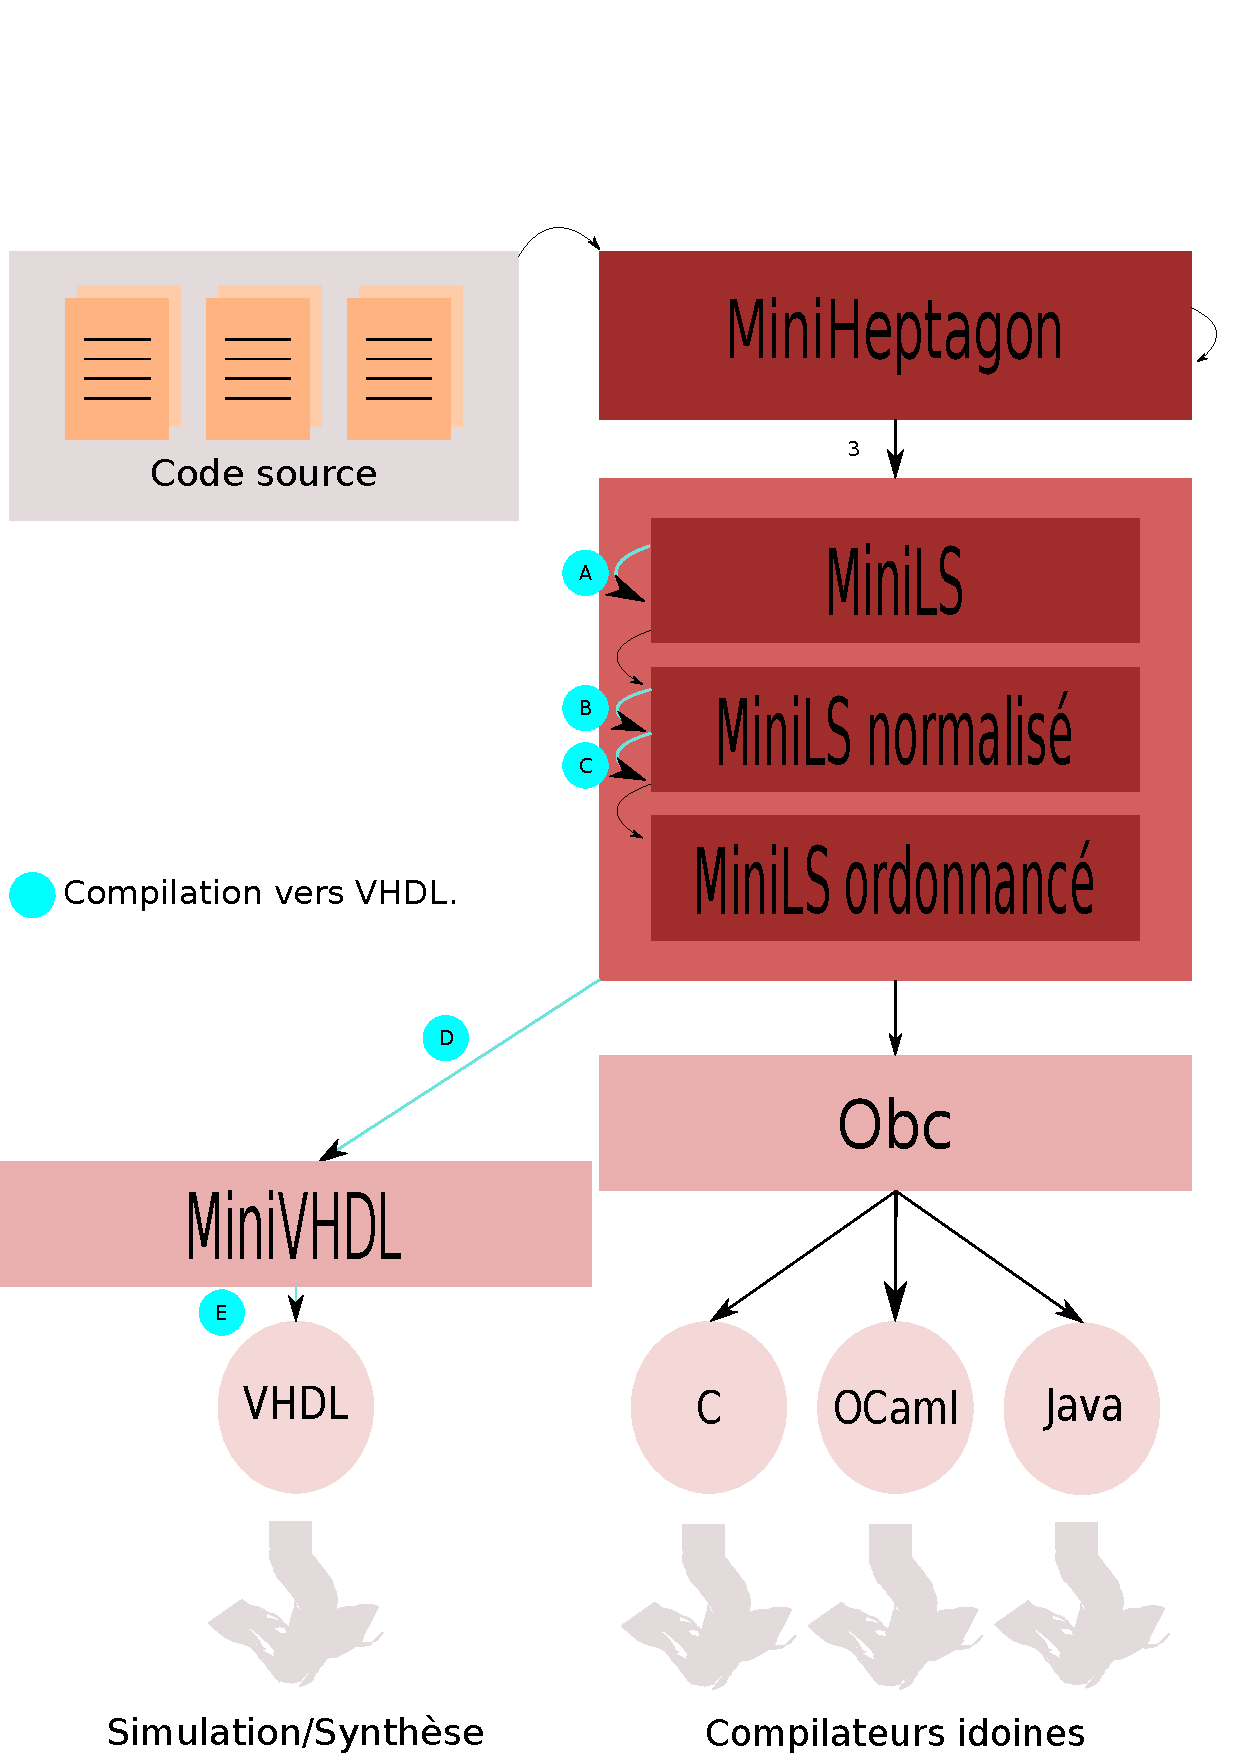
\includegraphics[scale=0.5]{archi}
  \caption{Architecture du compilateur \LANG}
  \label{fig:archi}
\end{figure}

Le passage au code s\'equentiel est court-circuit\'e lors d'une
compilation vers \vhdl, qui traduit \minils{} directement vers
celui-ci. Pour faciliter cette \'etape, trois simplifications sont
appliqu\'ees sur le code \minils.

\renewcommand{\labelenumi}{\Alph{enumi}.}
\begin{enumerate}
\item suppression de la r\'einitialisation logique;
\item suppression des it\'erateurs par expansion de code;
\item introduction d'une variable interm\'ediaire pour chaque argument d'un appel
  de noeud.
\end{enumerate}
\renewcommand{\labelenumi}{\arabic{enumi}.}

Le code obtenu sera finalement traduit vers un sous-ensemble de \vhdl, appel\'e
\minivhdl (\`a l'\'etape D), pr\^et \`a \^etre trait\'e par les outil d\'edi\'es (\'etape
E). Remarquons qu'il n'existe pas de d\'efinition pr\'ecise identifiant un
sous-ensemble ``synth\'etisable'' du langage \vhdl, g\'er\'e par les principaux outils
industriels. Apr\`es \'echange avec les partenaires du projet GENCOD, \minivhdl{}
nous parait maintenant correspondre \`a un sous-ensemble ``raisonnable'' de
\vhdl.


\section{De \LANG{} \`a VHDL}
Apr\`es avoir rappel\'e bri\`evement la forme des langages d'entr\'ee et de sortie, on
va expliciter la proc\'edure de traduction retenue.

\subsection{Langages internes}

\subsubsection{MiniLS}
\label{sec:syn:mls}

\begin{figure}[h]
  \centering
  \begin{eqnarray*}
    td & \Coloneqq & \mybox{type } bt = C + \dots + C \\
    d & \Coloneqq & \Node{p}{p}{p}{D} \\
    p & \Coloneqq & x : bt; \dots; x : bt \\
    D & \Coloneqq & pat = e; \dots; pat = e \\
    pat & \Coloneqq & x \p (pat,\dots,pat) \\
    e & \Coloneqq & x \p v \p \Op{e}{e} \p \Fby{v}{e} \p \Pre{e} \\
    & \p & \Every{f}{e}{e}{x} \p \When{e}{C}{x} \\
    & \p & \Merge{x}{C}{e}{C}{e} \\
    & \p & \Map{f}{e_1}{e_n} \\
    & \p & \Fold{f}{e_1}{e_n} \\
    & \p & \Mapfold{f}{e_1}{e_n} \\
    v & \Coloneqq & i \p C \\
    ck & \Coloneqq & \Base \p \On{ck}{C}{x}
  \end{eqnarray*}
  \caption{\minils}
  \label{fig:mls}
\end{figure}

\minils{} est un langage data-flow synchrone dans l'esprit de
\lustre~\cite{lustre:ieee91}, auquel on adjoint une construction de
r\'einitialisation modulaire et d'\'ecrire des \'equations gard\'ees par une
horloge. La compilation de \minils{} vers \vhdl{} passe successivement
par trois formes distinctes.

\begin{enumerate}
\item La forme originale (dont la syntaxe est d\'efinie dans la
  figure~\ref{fig:mls}) telle qu'obtenue \`a partir du code \LANG{}
  original.
\item Le code est traduit vers une forme normale
  (figure~\ref{fig:mlsn}).
\item La forme finale (voir figure~\ref{fig:mlsns}) est une forme
  normalis\'ee et dans laquelle les r\'einitialisations et les it\'erateurs
  de tableaux ont \'et\'e \'elimin\'es. De plus, les param\`etres effectifs des
  appels de fonctions sont n\'ecessairement des noms de variables.
\end{enumerate}

\begin{figure}[htp]
  \centering
  \begin{eqnarray*}
    e & \Coloneqq & x \p v \p \Op{e}{e} \p \When{e}{C}{x} \\
    ce & \Coloneqq & e \p \Merge{x}{C}{ce}{C}{ce} \\
    eq & \Coloneqq & x = ce \p x = \Fby{v}{e} \p x = \Pre{e} \\
    & \p & (x,\dots,x) = \Every{f}{e}{e}{x} \\
    & \p & (x,\dots,x) = \App{f}{e,\dots,e} \\
    & \p & (x,\dots,x) = \Map{f}{e_1}{e_n} \\
    & \p & (x,\dots,x) = \Fold{f}{e_1}{e_n} \\
    & \p & (x,\dots,x) = \Mapfold{f}{e_1}{e_n}
  \end{eqnarray*}
  \caption{\minils{} normalis\'e}
  \label{fig:mlsn}
\end{figure}

\begin{figure}[htp]
  \centering
  \begin{eqnarray*}
    e & \Coloneqq & x \p v \p \Op{e}{e} \p \When{e}{C}{x} \\
    ce & \Coloneqq & e \p \Merge{x}{C}{ce}{C}{ce} \\
    eq & \Coloneqq & x = \Pre{e} \\
    & \p & (x,\dots,x) = \App{f}{x,\dots,x}
  \end{eqnarray*}
  \caption{\minils{} simplifi\'e (et normalis\'e)}
  \label{fig:mlsns}
\end{figure}

\subsection{S\'emantique intuitive}
La s\'emantique de \minils{} est celle de \lustre: un noeud est compos\'e
d'un ensemble d'\'equa\-tions de suites mutuellement r\'ecursives. Discutons
des points qui distinguent le langage de \lustre:

\begin{enumerate}
\item Chaque expression $e$ est annot\'ee par une expression d'horloge
  $ck$. $e$ doit \^etre calcul\'ee lorsque $ck$ est vrai. Cette annotation
  est produite automatiquement par le compilateur au cours du calcul
  d'horloges.
\item $\Every{f}{e_1}{e_n}{x}$ permet de r\'einitialiser l'appel de
  noeud $f^{ck}(e_1,...,e_n)$ lorsque $e$ est vraie.
\item
%% Les expressions simples du langage s'ex\'ecutent uniquement dans l'instant, et
%% n'ont pas d'effet en dehors de celui-ci.

%% \[
%% \begin{array}{|r|llllllllllllllllllllllllllll}
%%   \hline
%%   1     & 1 & 1 & 1 & 1 & \dots \\
%%   \hline
%%   1 + 2 & 3 & 3 & 3 & 3 & \dots \\
%%   \hline
%% \end{array}
%% \]

%% \`A l'inverse, les expressions \textrm{pre} et \textrm{fby} permettent de retarder
%% leur argument d'un instant, avec une valeur d'initialisation dans le cas de
%% \textrm{fby}.

%% \[
%% \begin{array}{|r|llllllllllllllllllllllllllll}
%%   \hline
%%   1 \ \mathrm{fby} \ 2 & 1 & 2 & 2 & 2 & \dots \\
%%   \hline
%%   \mathrm{pre} \ 3 &  & 3 & 3 & 3 & \dots \\
%%   \hline
%% \end{array}
%% \]

  Les constructions \texttt{when} et \texttt{merge} permettent,
  appliqu\'ees \`a des expressions, de sous-\'echantillon\-ner et
  sur-\'echantillonner ces derni\`eres. L'emploi de ces constructions a un
  effet sur les horloges: l'horloge de $\When{e}{C}{x}$ est
  $\On{ck}{C}{x}$, o\`u $ck$ est celle de $e$, et l'horloge de
  $\Merge{x}{C_1}{e_1}{C_n}{e_n}$ est $ck$ quand celle des $e_i$ est
  $\On{ck}{C}{x}$. L'expression $\On{ck}{C}{x}$ indique que le
  r\'esultat est pr\'esent lorsque l'horloge $ck$ est vraie et que $x$ est
  \'egal \`a $C$.

\[
\begin{array}{r|llllllllllllllllllllllllllll}
  \hline
  x & 1 & 2 & 3 & 4 & \dots \\
  \hline
  h & false & true & false & true & \dots \\
  \hline
  \When{x}{true}{h} & & 2 & & 4 & \dots \\
  \hline
  u &  & 1 & & 4 & \dots \\
  \hline
  v & 0 & & 3 & & \dots \\
  \hline
  \Merges{h}{true}{u}{false}{v} & 0 & 1 & 3 & 4 \\
  \hline
\end{array}
\]

\item
Les it\'erateurs \texttt{map}, \texttt{fold}, et \texttt{mapfold}
prennent en argument une fonction $f$, une taille de tableau et un ou
plusieurs tableaux. La s\'emantique de ces constructions est celle
donn\'ee dans~\cite{lucy:genie00,morel-07-jes}.

\begin{itemize}
\item \texttt{map} applique en parall\`ele $f$ \`a tous les \'el\'ements des tableaux
  pour former un nouveau tableau.
\item \texttt{fold} applique en s\'erie $f$ sur tous les \'el\'ements d'un tableau en
  passant un accumulateur et renvoie ce dernier une fois le parcours termin\'e.
\item \texttt{mapfold}, qui suppose que $f$ renvoie au moins deux valeurs,
  combine les deux en construisant un nouveau tableau avec le premier r\'esultat
  de $f$ (\`a la mani\`ere de \texttt{map}) et en passant un accumulateur durant le
  parcours (tout comme \texttt{fold}).
\end{itemize}
\end{enumerate}

\subsubsection{MiniVHDL}

\minivhdl{} (d\'efini dans la figure~\ref{fig:mvhdl})
est un fragment de \vhdl{} suffisant pour
d\'ecrire l'essence du processus de traduction. Un composant \minivhdl:
\[
\Component{f}{P}{sigs}{lvars}{ports}{I}
\]
correspond \`a un
composant \vhdl{} form\'e des instantiations $ports$, signaux internes $sigs$ et d'un
processus avec les variables locales $lvars$ et de corps $I$.

Le langage est structur\'e sous forme de composants. Chacun d'eux poss\`ede des
signaux d'entr\'ee et de sortie, des signaux locaux, des variables locales, d'\'eventuels
sous-composants, et enfin un corps form\'e d'une suite d'instructions.

La s\'emantique informelle du langage est la suivante: d\`es que la valeur d'un
signal d'entr\'ee ou local change, le corps du composant est ex\'ecut\'e. Celui-ci
peut modifier la valeur d'autres signaux via l'instruction $x \Leftarrow e$ ($x$
\'etant par d\'efinition un signal), entra\^{\i}nant ainsi l'activation de
sous-composants, ou m\^eme la r\'eactivation du composant courant. Les variables
locales sont semblables aux variables des langages de programmation
traditionnels: elles n'ont de valeur que pendant l'ex\'ecution du corps d'un
composant. L'ex\'ecution s'arr\^ete une fois tous les signaux stables.

\begin{figure}[t]
  \centering
  \begin{eqnarray*}
    component & \Coloneqq & \mybox{component} \; f \; \mybox{port} \; sm;\dots;\
    sm \; \mybox{with} \, \mybox{sig} \; d; \dots; d \; \\
    & & \mybox{and} \, \mybox{var} \; d; \dots; d \; \mybox{and} \
    \mybox{subcomponents} \; p; \dots; p \; \mybox{in} \; I \\
    sm & \Coloneqq & x : mode \ ty \\
    sd & \Coloneqq & x : mode \ ty := e \\
    mode & \Coloneqq & \mybox{in} \p \mybox{out} \\
    d & \Coloneqq & x : ty \\
    p & \Coloneqq & \mybox{port map } x (bd;\dots;bd) \\
    bd & \Coloneqq & x \Rightarrow x \\
    I & \coloneqq & i; \dots; i \\
    i & \Coloneqq & \Assign{x}{e} \p \Affect{x}{e} \p \Case{e}{v}{I}{v}{I} \\
    e & \Coloneqq & id \; \vert \; v \; \vert \; \Op{e}{e} \\
    v & \Coloneqq & i \; \vert \; ' bitp ' \\
    bitp & \Coloneqq & bit \p bit \  bitp \\
    bit & \Coloneqq & \mathbf{0} \p \mathbf{1} \\
    bt & \Coloneqq & \mybox{natural} \p \mybox{std\_logic} \p \mybox{bit}
    \p \dots
  \end{eqnarray*}
  \caption{MiniVHDL}
  \label{fig:mvhdl}
\end{figure}

Notons que les param\`etres effectifs des sous-composants sont des noms de
signaux; cela justifie la forme simplifi\'ee \minils{} d\'ecrite pr\'ec\'edemment.

\subsection{Simplification de MiniLS normalis\'e}

Nous effectuons donc trois passes pour simplifier le code \minils.

\subsubsection{\'Elimination de la r\'einitialisation logique}

Comme expliqu\'e plus haut, certaines constructions de \minils{} proposent au
programmeur une forme de r\'einitialisation modulaire : les \'equations de la
forme $\Fby{v}{e}$ d'un noeud $f$ instanci\'e par la construction
$\Every{f}{e_1}{e_n}{z}$ doivent \^etre r\'einitialis\'ees d\`es lors que $z$
est vrai.

La premi\`ere passe de simplification, qui s'ex\'ecute sur le code \minils{}
obtenu \`a la troisi\`eme \'etape du processus d\'ecrit plus haut, va exprimer
la r\'einitialisation en fonction du reste du langage, r\'eduisant ainsi la
complexit\'e du langage \`a traduire vers \vhdl{}.

On va supposer dans ce qui suit que l'identificateur \textbf{rst} est un
identificateur utilis\'e nulle part dans le programme. En pratique, le compilateur
s'assure de l'absence de conflit avec les variables de l'utilisateur.

L'id\'ee est d'ajouter \`a chaque noeud un argument suppl\'ementaire nomm\'e
\textbf{rst} qui vaudra $true$ lorsqu'une r\'einitialisation de la m\'emoire est
n\'ecessaire, et de modifier les expressions contenant des constructions
\texttt{fby} ou \texttt{every} pour prendre en compte \textbf{rst}. L'exemple
suivant reprend le compteur simple pr\'esent\'e plus haut pour illustrer cette
simplification.

\verbatiminput{rst_ex.ept}

Une fois le reset \'elimin\'e, le code est le suivant :

\verbatiminput{rst_ex2.ept}

On va d\'etailler les fonctions effectuant ces deux t\^aches : $RstE(e)$ prend
une expression \minils{} $e$ et renvoie une nouvelle expression o\`u la
r\'einitialisation a \'et\'e \'elimin\'ee, et $RstNode(nd)$ prend un noeud $nd$
et renvoie un nouveau noeud prenant un \texttt{rst} \`a un noeud et transforme
ses \'equations.

\newcommand{\re}[1]{RstE(#1)}
\newcommand{\rstn}[1]{RstNode(#1)}

\[
\begin{array}{lcl}
  \re{\Op{e_1}{e_n}} & = & \Op{\re{e_1}}{\re{e_n}} \\
  \re{\Fby{v}{e}} & = & \If{rst}{v}{(\Fby{v}{\re{e}})} \\
  \re{\Pre{e}} & = & \Pre{\re{e}} \\
  \re{\Every{f}{e_1}{e_n}{x}} & = & \App{f}{\mathbf{rst} \; \mathtt{or} \;
    x, \re{e_1} \dots, \re{e_n}} \\
  \re{\App{f}{e_1,\dots,e_n}} & = &
  \App{f}{\mathbf{rst},\re{e_1},\dots,\re{e_n}} \\
  \re{\If{e_1}{e_2}{e_3}} & = & \If{\re{e_1}}{\re{e_2}\\ & & \hspace{1.9cm}}
  {\re{e_3}} \\
  \re{\When{e}{C}{x}} & = & \When{\re{e}}{C}{x} \\
  \re{\Merge{e}{C_1}{e_1}{C_n}{e_n}} & = &
  \mybox{merge} \; \re{e} \; (C_1 \Rightarrow \re{e_1}) \\
  & & \hspace{2.4cm} \dots \\
  & & \hspace{2.4cm} (C_n \Rightarrow \re{e_n})
\\ \\
RstEqs(pat_1 = e_1;\dots;pat_n = e_n) & = &
  pat_1 = \re{e_1};\dots;pat_n = \re{e_n} \\
  \end{array}
\]

\[
\begin{array}{ll}
  \rstn{\Node{f}{x_1,\dots,x_n}{y_1,\dots,y_n}{eqs}} & = \\
  \ind \Node{f}{rst,x_1,\dots,x_n}{y_1,\dots,y_n}{ResetEqs(eqs)}
\end{array}
\]

\subsubsection{Suppression des it\'erateurs}

La version actuelle du compilateur et de son g\'en\'erateur de code \vhdl{} supporte
les tableaux de dimension arbitraire \footnote{En pratique, les outils de
  synth\`ese de circuits \`a partir de code \vhdl{} imposent une dimension maximale.}
et constructions associ\'ees ; il nous faut donc compiler les it\'erateurs
\texttt{map}, \texttt{fold} et \texttt{mapfold} vers \vhdl{}.

Par souci de simplicit\'e et uniformit\'e, nous avons fait le choix de les
\'eliminer par expansion lors d'une transformation source-\`a-source sur
\minils. On ne d\'etaillera pas cette op\'eration qui consiste simplement \`a
remplacer les it\'erateurs par plusieurs \'equations. L'\'equation $x =
\Map{f}{t_1}{t_m}$ lorsque les tableaux $t_1, \dots, t_m$ sont de taille $n$
sera ainsi remplac\'ee par $n + 1$ \'equations dont les $n$ premi\`eres
effectuent l'application de $f$ pour chaque indice et la derni\`ere affecte \`a
$x$ le tableau en r\'esultant. On applique des transformations similaires aux
op\'erateurs \texttt{fold} et \texttt{mapfold}.

Le programme suivant pr\'esente un exemple effectuant un ET logique sur tous les
\'el\'ements d'un tableau via l'it\'erateur \texttt{fold}.

\verbatiminput{fold_orig.ept}

Son pendant avec it\'erateur mis \`a plat se contente de passer l'accumulateur
d'\'el\'ement en \'el\'ement.

\verbatiminput{fold_il.ept}

Un traitement sp\'ecial est adopt\'e pour l'utilisation de \texttt{map} avec
certains op\'erateurs. En effet, \vhdl{} permet d'utiliser certains op\'erateurs sur
des tableaux de bits, sans avoir \`a d\'econstruire ces derniers ; par exemple, il
est possible d'effectuer un ET logique bit-\`a-bit sur deux tableaux $t_1$ et
$t_2$ via $t_1 \ \texttt{and} \ t_2$. La passe effectue la transformation de
$\texttt{map}\ \textbf{op}<<n>>(t_1,\dots,t_n)$ \`a $t_1\ \textbf{op}\ \dots
\textbf{op}\ t_n$ lorsque cela est possible.

\subsubsection{Simplification des appels}

\newcommand{\simpl}[2]{Simpl(#1,#2)}
\newcommand{\simplnd}[1]{SimplNode(#1)}

Comme nous le verrons plus loin, les appels de noeuds seront compil\'es
en instantiations de composants. Or, les arguments d'une construction
\vhdl{} $port \; map$ sont forc\'ement des identificateurs. Afin de
simplifier la g\'en\'eration de \vhdl{}, nous modifiont en amont chaque
appel de noeud en introduisant une variable interm\'ediaire pour chaque
argument. La fonction $\simpl{eq}{eqs}$ simplifie l'\'equation $eq$ en
ajoutant la (ou les) \'equation(s) produite(s) \`a la liste des \'equations
d\'ej\`a trait\'ees $eqs$ ; $\simplnd{nd}$ prend un noeud $nd$ et simplifie
les appels pr\'esents dans ses \'equations. L'op\'eration ($\Cons$) d\'esigne
la concat\'enation en t\^ete de liste.

\[
\begin{array}{ll}
  \simpl{x = ce}{eqs} & = \\
  \ind (x = ce) \Cons eqs \\
  \simpl{x = \Pre{e}}{eqs} & = \\
  \ind (x = \Pre{e}) \Cons eqs \\

  \simpl{(x_1,\dots,x_n) = \App{f}{e_1,\dots,e_n}}{eqs} & = \\
  \ind (y_1 = e_1) \Cons \dots \Cons (y_n = e_n)
  \Cons ((x_1,\dots,x_n) = \App{f}{rst,y_1,\dots,y_n}) \Cons eqs \\
  \ind \mbox{o\`u } y_1,\dots,y_n \mbox{ sont des noms de variables frais}
\end{array}
\]

\[
\begin{array}{ll}
  \simplnd{\Node{x_1,\dots,x_n}{y_1,\dots,y_n}{p}{D}} & = \\
  \ind \mathtt{node} f(x_1,\dots,x_n) = y_1, \dots, y_n \; \\
  \ind \mathtt{with} \  \mathtt{var} \; p' \; \mathtt{in} \; fold\_right \;Simpl
  \; D \; [] \\
  \ind \mbox{en supposant que $p'$ correspond
             aux variables d\'efinies par} \\ \ind \mbox{les nouvelles \'equations.}
\end{array}
\]

Ces simplifications effectu\'ees, le programme r\'esultant est traduit vers \minivhdl.

\subsection{MiniLS simplifi\'e vers MiniVHDL}

Le principe g\'en\'eral de la traduction de \minils{} simplifi\'e vers
\minivhdl{} est le suivant:

\begin{enumerate}
\item La traduction est appliqu\'ee au corps d'un noeud, c'est-\`a-dire
un syst\`eme d'\'equation ordonnanc\'e.
\item Chaque noeud \minils{} correspond \`a un composant \minivhdl.
\item Chaque \'equation \`a m\'emoire (i.e. contenant $fby$ ou $pre$) correspond
  \`a un signal \vhdl{} local et
  chaque \'equation combinatoire \`a la d\'efnition d'une variable locale
  (une affectation en \vhdl).
\item Les horloges importent uniquement pour les \'equations de la forme:
\[
\begin{array}{c}
x = \Fby{v}{e}
\end{array}
\mbox{ et }
\begin{array}{c}
(x_1,\dots,x_n) = \App{f}{e_1,\dots,e_n}
\end{array}
\]
Il faut cependant g\'en\'erer la garde bool\'eenne correspondant \`a l'horloge
logique $ck$. Les autres \'equations, m\^eme si elles sont gard\'ees par une
horloge sont combinatoires et ne n\'ecessitent pas de traitement
particulier.
\item La r\'einitialisation logique est g\'er\'ee en amont comme expliqu\'ee ci-dessus,
  elle est donc implicitement asynchrone (ind\'ependante des fronts montants de
  l'horloge).
\item Les partenaires ont exprim\'e le d\'esir de pouvoir r\'einitialiser
  physiquement toute la m\'emoire lors du basculement d'un signal pr\'ecis
  nomm\'e \textbf{hwrst} (pour ``hardware reset''). Nous ajoutons donc
  un signal suppl\'ementaire dans dans le code \minils{} et on g\'en\`ere le
  code de r\'einitialisation correspondant lors du traitement du
  $fby$. Tout comme pour l'identificateur \textbf{rst} plus haut, on
  suppose que l'identificateur \textbf{hwrst} n'est pas utilis\'e dans
  le programme (un renommage pr\'ealable permet de l'assurer).
\item Pour respecter la s\'emantique \`a $\Delta$-cycles de \vhdl{}, il importe de
  faire \'evoluer la m\'emoire par un pas du calcul uniquement sur front montant de
  l'horloge.
\item En suivant le mod\`ele synchrone, les valeurs calcul\'ees par le circuit \`a
  d'autres moments que le front montant n'ont pas de sens bien d\'efini ; on les
  ignorera donc.
\item Chaque appel de noeud correspondra \`a une instantiation. Comme
  sp\'ecifi\'e plus haut, les param\`etres effectifs d'un signal \vhdl{}
  sont obligatoirement des signaux auxquels il faudra assigner la
  valeur correcte.
\end{enumerate}

\subsubsection{Traduction des types}

Les d\'eclarations de types de donn\'ees ont \'et\'e laiss\'ees implicites aussi
bien dans la syntaxe de \minils{} que de \minivhdl{} ; les
possibilit\'es \'etant exactement les m\^emes (\'enum\'erations et
enregistrements), on choisit de ne pas s'attarder sur leur traduction
qui reste une traduction mot-\`a-mot d'une syntaxe concr\`ete \`a l'autre.

\subsubsection{Traduction des constantes et fonction auxiliaires sur les horloges}

La fonction $TradConst(c)$ traduit une constante \minils{} $c$ en constante
\minivhdl{}.

\newcommand{\TradC}[1]{TradConst(#1)}

\[
\begin{array}{lcl}
  \TradC{i} & = & i \\
  \TradC{true} & = & '1' \\
  \TradC{false} & = & '0' \\
  \TradC{C} & = & C
\end{array}
\]

La fonction auxiliaire $GuardClock$ permet de traduire une horloge \minils{} en
expression \minivhdl{} de type bool\'een. Elle sera utilis\'ee pour contr\^oler la
mise \`a jour des registres, s'assurant que cette derni\`ere n'est effectu\'ee
qu'aux instants o\`u l'horloge est effective.

\newcommand{\GEC}[1]{GuardClock(#1)}

\[
\begin{array}{lcl}
  \GEC{\Base} & = & rising\_edge(clk) \\
  \GEC{\On{ck}{C}{x}} & = & x = \TradC{C} \; \mathtt{and} \; \GEC{ck}
\end{array}
\]

Tout comme les mises \`a jour des m\'emoires, les appels \`a d'autres noeuds
sont dirig\'es par les horloges qui en donnent la cadence. Il nous faudra donc
une fonction voisine de $GuardClock$ pour calculer l'expression \minivhdl{}
correspondant \`a l'horloge utilis\'ee dans l'appel d'un noeud.

\newcommand{\EC}[1]{ExpClock(#1)}

\[
\begin{array}{lcl}
  \EC{\Base} & = & clk \\
  \EC{\On{ck}{C}{x}} & = & x = \TradC{C} \; \mathtt{and} \; \EC{ck}
\end{array}
\]

\subsubsection{Traduction des expressions et \'equations}

La fonction $TradExp(e)$ traduit l'expression \minils{} normalis\'ee et
simplifi\'e $e$ en expression \minivhdl{}.

\newcommand{\TradE}[1]{TradExp(#1)}

\[
\begin{array}{lcl}
  \TradE{v} & = & \TradC{v} \\
  \TradE{x} & = & x \\
  \TradE{\Op{e_1}{e_n}} & = & \Op{\TradE{e_1}}{\TradE{e_n}} \\
  \TradE{\When{e}{C}{x}} & = & \TradE{e}
\end{array}
\]

La construction \texttt{when} n'a pas de sens calculatoire, et peut n'\^etre vue
que comme une annotation d'horloge. Elle sera ignor\'ee lors du processus de
traduction.

La fonction $TradCExp(ce)$ traduit les expressions $ce$ de contr\^ole form\'ees
d'expressions simples ou de \texttt{merge} imbriqu\'es en instructions \minivhdl{}.

\newcommand{\TradCE}[2]{TradCExp(#1, #2)}

\[
\begin{array}{ll}
  \TradCE{x}{\Merge{y}{C_1}{ce_1}{C_n}{ce_n}} & = \\
  \ind \mathtt{case} \; y \; \mathtt{of} \;
  (\TradC{C_1} \Rightarrow \TradCE{x}{ce_1}) \\
  \hspace{2.1cm} \dots \\
  \hspace{2.1cm} (\TradC{C_n} \Rightarrow \TradCE{x}{ce_n}) \\
  \TradCE{x}{e} & = \\
  \ind \Affect{x}{\TradE{e}}
\end{array}
\]

Enfin, la fonction $TradEq$ permet de passer des \'equations aux
instructions \minivhdl{}. Elle prend un argument suppl\'ementaire
permettant de compter le nombre d'appels de noeuds afin de g\'en\'erer des
arguments suppl\'ementaires, et on se donne une fonction suppl\'ementaire
$MakeArg(x,i)$ qui g\'en\`ere un nom de variable frais \`a partir du nom de
variable $x$ et de l'entier $i$.

La traduction des \'equations appelant un noeud n\'ecessite des
explications concernant la fa\c{c}on de compiler les appels d'un noeud
\minils{} qui seront donn\'ees \`a la section suivante.

\newcommand{\TradEq}[2]{TradEq(#1,#2)}
\newcommand{\MA}[2]{MakeArg(#1,#2)}

\[
\begin{array}{lcl}
  \TradEq{x = ce}{i} & = & \TradCE{x}{ce}, i \\

  \TradEq{x = \Pre{e}}{i} & = & \mathtt{if} \; \GEC{ck} \; \mathtt{then} \\
  & & \ind \Assign{x}{\TradE{e}} \\
  & & \mathtt{end} \; \mathtt{if}, i \\

  \TradEq{x = \Fby{y}{e}}{i} & = & \mathtt{if} \; \mathbf{hwrst}
  \; \mathtt{then} \\
  & & \ind \Assign{x}{y} \\
  & & \mathtt{elsif} \; \GEC{ck} \; \mathtt{then} \\
  & & \ind \Assign{x}{\TradE{e}} \\
  & & \mathtt{end} \; \mathtt{if}, i \\


  \TradEq{(x_1,\dots,x_n) = \App{f}{y_1,\dots,y_n}}{n} & = &
  \Assign{\MA{"ck"}{i}}{\EC{ck}} \\
  & & \Assign{\MA{y_1}{i}}{y_1} \\
  & & \dots \\
  & & \Assign{\MA{y_n}{i}}{y_n}, i + 1 \\
\end{array}
\]

Pr\'ecisons que par construction, l'interface d'un composant suit toujours la
forme suivante:
\[(clk, hwrst, in_1, \dots,in_n, out_1,\dots,out_n)
\]
Rappelons que le reset ``logique'' (celui utilis\'e dans les automates,
par exemple ou la construction \verb-every-) est maintenant une entr\'ee
suppl\'ementaire (ici $in_1$).

\subsubsection{Gestion des tableaux}

Hormis le cas des it\'erateurs trait\'es pr\'ec\'edemment, la gestion des
tableaux n'appelle pas de commentaire particulier, \`a l'exception de la
n\'ecessit\'e de d\'eclarer \`a l'avance les types tableaux (bornes exclues) en
\vhdl{}. Deux solutions sont envisageables:

\begin{enumerate}
\item Calculer la dimension maximale des tableaux rencontr\'es dans le
  programme, et utiliser cette information pour pr\'e-d\'eclarer les
  tableaux \vhdl{} idoines.
\item D\'eclarer quoi qu'il advienne les types de tableaux utiles et
  refuser les programmes comprenant des dimensions sup\'erieures \`a une
  limite fix\'ee \`a l'avance.
\end{enumerate}

Le compilateur emploie pour l'instant la premi\`ere m\'ethode mais la seconde ne
nous semble pas d\'erangeante pour des raisons pragmatiques~\footnote{Notons que
  notre version de l'outil Xilinx ISE refuse tout tableau de
  dimension sup\'erieure \`a trois.}.

\subsubsection{Compilation modulaire et appels de noeuds}

\minivhdl{} offre une forme de modularit\'e bas\'ee sur une hi\'erarchie de
composants. Chacun de ces derniers sp\'ecifie une liste de composants fils dont
les ports (au sens de la figure \ref{fig:mvhdl}) sont instanti\'es avec des
signaux. Nous prenons donc soin d'utiliser des signaux comme r\'esultats mais
aussi comme arguments. Par souci de simplicit\'e, on introduit des signaux locaux
pour chaque argument, signaux qui seront affect\'es lors de la traduction de
l'\'equation correspondant \`a l'appel de noeud original.

La fonction $GatherPortMaps(D, i)$ rassemble cette liste de sous-noeuds \`a
partir des appels de noeud pr\'esents dans le paquet d'\'equations $D$ et
cr\'e\'e les instantiations de composants correspondantes. L'entier $i$ nous
servira \`a distinguer les appels de noeuds et de cr\'eer de nouveaux noms de
signaux frais gr\^ace \`a la fonction $MakeArg$ d\'ecrite plus haut. On se donne
\'egalement une fonction $GetArgName(f,n)$ qui renvoie le nom du $n$-\`eme
argument du noeud de nom $f$.

\newcommand{\GPM}[2]{GatherPortMaps(#1,#2)}
\newcommand{\GAN}[2]{GetArgName(#1,#2)}

\[
\begin{array}{lcl}
  \GPM{[]}{i} & = & [] \\
  \GPM{((x_1,\dots,x_n) = \App{f}{y_1,\dots,y_n}) \Cons eqs}{i} & = &
  \\
  \ind \mybox{port map} \; f ( clk \Rightarrow \MA{"clk"}{i} \\
  \ind \ind \ind \ind \hspace{0.4cm} \GAN{f}{1} \Rightarrow \MA{y_1}{i} \\
  \ind \ind \ind \ind \hspace{0.4cm} \dots \\
  \ind \ind \ind \ind \hspace{0.4cm} \GAN{f}{n} \Rightarrow \MA{y_n}{i}) \\
  \ind \Cons \GPM{eqs}{i + 1}
\end{array}
\]

On d\'efinit ensuite les fonctions auxiliaires $NeedVar$, $Vars$,
$ParamSigs$ et $SignalOfVarDec$ respectivement charg\'ees de d\'eterminer
si une \'equation introduit des d\'eclarations de variables locales ou
non, de calculer la liste des variables d\'efinies par une \'equation, de
calculer les signaux \`a passer en arguments aux appels de noeuds
pr\'esents dans un paquet d'\'equations et enfin de traduire simplement
une d\'eclaration de variable \minils{} en d\'eclaration de signal
\minivhdl{} avec mode d'utilisation (entr\'ee ou sortie).

\newcommand{\NV}[1]{NeedVar(#1)}
\newcommand{\V}[1]{Vars(#1)}
\newcommand{\PS}[2]{ParamSigs(#1,#2)}
\newcommand{\SoVD}[3]{SignalOfVarDec(#1 : #2, #3)}

\[
\begin{array}{lcl}
  \NV{x = \Fby{v}{e}} & = & false \\
  \NV{(x_1,\dots,x_n) = \App{f}{y_1,\dots,y_n}} & = & false \\
  \NV{x = ce} & = & true
\end{array}
\]

\[
\begin{array}{lcl}
  \V{x = \Fby{v}{e}} & = & [x] \\
  \V{(x_1,\dots,x_n) = \App{f}{y_1,\dots,y_n}} & = & x_1 \Cons \dots \Cons x_n \\
  \V{x = ce} & = & [x]
\end{array}
\]

\[
\begin{array}{ll}
  \PS{x = \Fby{v}{e} \Cons eqs}{i} & = \\
  \ind \PS{eqs}{i} \\
  \PS{(x_1,\dots,x_n) = \App{f}{y_1,\dots,y_n} \Cons eqs}{i} & = \\
  \ind \MA{"clk"}{i} \Cons \MA{y_1}{i} \Cons \dots \Cons \MA{y_n}{i} \\
  \ind \mathtt{::} \; \PS{eqs}{i + 1}
  \\
  \PS{x = ce \Cons eqs}{i} & = \\
  \ind \PS{eqs}{i}
\end{array}
\]

\[
\begin{array}[lcl]{lcl}
  \SoVD{x}{bt}{mode} & = & \mybox{signal} \; x : mode \; TransBaseType(bt)
\end{array}
\]

\subsubsection{Traduction des noeuds}

Enfin, $TradNode(nd)$ se charge de traduire un noeud $nd$ en composant
\minivhdl{}, en cr\'eant un signal local pour chaque \'equation retard\'ee et
argument d'appel de noeud, une variable pour chaque \'equation combinatoire, et
la liste de sous-composants requise.

\begin{align*}
  & TradNode(\mybox{node } f(in) = out \mybox{ with var } p \mybox{ in } D) = \\
  & \bl \mbox{soit } port = \\
  & \bl \bl clk : \mybox{in std\_logic}; \\
  & \bl \bl \{ SignalOfVarDec(x : bt, \mybox{in}) \p (x : bt) \in in \}; \\
  & \bl \bl \{ SignalOfVarDec(x : bt, \mybox{out}) \p (x : bt) \in out \}, \\
  & \bl \mbox{ soit } signals = \{ \V{eq} \p eq \in D, \neg \NV{eq} \}
  \mybox{,} \\
  & \bl \mbox{ soit } sig\_args = \PS{D}{1} \mybox{,} \\
  & \bl \mbox{ soit } variables = \{ \V{eq} \p eq \in D, \NV{eq} \} \mybox{,} \\
  & \bl \mbox{ soit } ports = \GPM{D}{1} \mybox{,} \\
  & \bl \mbox{ soit } body = fold\_right TradEq D ([], 1) \mbox{ dans} \\
  & \mybox{component } f \mybox{ port } port \mybox{ with sig } signals \cup
  sig\_args \\
  & \mybox{and var } variables \mybox{ and subcomponents } ports \mybox{ in }
  body
\end{align*}

L'impl\'ementation suit fid\`element les \'etapes d\'ecrites ici. Ces fonctions
ont \'et\'e impl\'ement\'ees dans le compilateur \heptagon{}. Le code charg\'e de
la traduction de \minils{} vers \minivhdl{} est court (de l'ordre de
600 lignes de code OCaml). Notons que le compilateur r\'ealis\'e est
capable d'assurer le retour au source (tra\c{c}abilit\'e) depuis le code
\LANG{} (conservation des identificateurs et de leur renommage au
cours des \'etapes de compilation). L'ensemble du compilateur fait de
l'ordre de 15000 lignes de code Ocaml.

\section{Conclusion}

Ce document a d\'ecrit une m\'ethode de compilation d'un langage
synchrone proche de \scade{} \`a partir d'une repr\'esentation interm\'ediaire
data-flow avec horloges. Le r\'esultat est une impl\'ementation d\'ecrite formellement
et particuli\`erement petite (en nombre de lignes de code). Nous pensons
que la technique propos\'ee ici pourrait \^etre int\'egr\'ee assez facilement
dans un compilateur tel que KCG \`a partir de son format interne interm\'ediaire
data-flow.

Plusieurs exemples fournis par les membres du projet ont \'et\'e
exp\'eriment\'es. L'efficacit\'e du code obtenu semble comparable au code
produit depuis le code C g\'en\'er\'e par le compilateur KCG.

\newpage
\tableofcontents

\newpage
\bibliographystyle{plain}
\bibliography{lucy,synchrone,biblio}

\newpage
\appendix


\section{Exemples de code g\'en\'er\'e}

On pr\'esente ici quelques codes g\'en\'er\'es par notre prototype. En l'\'etat
actuel de ce dernier, beaucoup de variables interm\'ediaires inutiles sont
g\'en\'er\'ees ; cela s'explique pour deux raisons :

\begin{itemize}
\item Ces codes repr\'esentent des sorties brutes n'ayant subies aucune
  optimisation.
\item Certaines passes du compilateur ont naturellement tendance \`a introduire
  des variables interm\'ediaire de fa\c{c}on pr\'eventive, simplifiant ainsi leur
  fonctionnement.
\end{itemize}

\subsection{Compteur}

\paragraph{MiniLS initial}

\small
\verbatiminput{compteur2_init.mls}
\normalsize

\paragraph{MiniLS normalis\'e, ordonnanc\'e et simplifi\'e}

Notons que le noeud \textit{compteur} est ici instanci\'e avec son param\`etre
\textit{n} \'egal \`a 4, ceci afin de pouvoir d\'eplier les it\'erateurs.

\small
\verbatiminput{compteur2_sched.mls}
\normalsize

\paragraph{VHDL}

\small
\verbatiminput{compteur2_vhdl.vhd}
\normalsize

\subsection{Allocateur de ressource}

\paragraph{MiniLS initial}

\small
\verbatiminput{al2_init.mls}
\normalsize

\paragraph{MiniLS normalis\'e, ordonnanc\'e et simplifi\'e}

\small
\verbatiminput{al2_sched.mls}
\normalsize

\paragraph{VHDL}

\small
\verbatiminput{al2_vhdl.vhd}
\normalsize

\section{Utilisation du compilateur}

Nous supposerons dans ce manuel que l'archive du compilateur a \'et\'e
d\'ecompress\'ee dans le r\'epertoire \verb/$HEPTDIR/. Cette archive contient le
pr\'esent rapport, un r\'epertoire \texttt{exs/} avec une batterie d'exemples
\LANG{} compil\'es vers \vhdl{}, et un binaire en code-octet pour la machine
abstraite OCaml. Ce dernier peut-\^etre ex\'ecut\'e via \texttt{ocamlrun heptc},
ou bien directement lorsque votre \texttt{ocamlrun} est pr\'esent dans
\texttt{/usr/bin}. Nous supposerons par la suite que c'est le cas et que votre
variable d'environnement \verb/$PATH/ contient \verb/$HEPTDIR//bin.

Pour utiliser le compilateur, il faut tout d'abord renseigner la variable
d'environnement \verb/$HEPTLIB/ sp\'ecifiant au compilateur o\`u trouver la
biblioth\`eque standard.

\begin{verbatim}
$ export HEPTLIB=$HEPTDIR/lib
\end{verbatim}

Vous pouvez ensuite v\'erifier que le compilateur est disponible et fonctionnel
via la commande suivante :

\begin{verbatim}
$ heptc -version
The Heptagon compiler, version 0.4 (wed. aug. 18 11:17:42 CET 2010)
Standard library in [...]
\end{verbatim}

Pour compiler un fichier \LANG, le compilateur doit \^etre invoqu\'e avec l'option
\verb/-target/. Les arguments possibles pour cette option sont :

\begin{itemize}
\item \verb/vhdl/ : g\'en\`ere du code \vhdl{}.
\item \verb/mls/ : g\'en\`ere le code \`a flots de donn\'ees \minils{} interm\'ediaire.
\item \verb/obc/ : g\'en\`ere un code imp\'eratif simple dans le langage id\'ealis\'e Obc.
\item \verb/c/ : g\'en\`ere du code C.
\end{itemize}

Les cibles \vhdl{} et C invoqu\'ees sur un fichier \verb/source.ept/ produisent
respectivement un dossier \verb/source_vhdl/ et \verb/source_c/ qui contiennent
les fichiers sources g\'en\'er\'es. Par exemple :

\begin{verbatim}
$ cat source.ept
node main() returns (o : int)
let
  o = 0 fby (o + 1);
tel
$ heptc -target vhdl source.ept
$ ls source_vhdl
main.vhd  types.vhd
\end{verbatim}

L'option \verb/-s noeud/ permet de g\'en\'erer le code n\'ecessaire \`a un
ex\'ecutable autonome \`a partir d'un fichier source \LANG, c'est \`a dire un
\textit{test-bench} dans le cas de \vhdl{} et une fonction \verb/main()/ en ce
qui concerne C. Voici un exemple d'utilisation de la sortie C :

\begin{verbatim}
$ cat source.ept
node noeud() returns (o : int)
let
  o = 0 fby (o + 1);
tel

node main() returns (o : int)
let
  o = noeud() + 1;
tel
$ heptc -target c -s main source.ept
$ ls source_c
_main.c  _main.h  source.c  source.h  source_types.c  source_types.h
$ cc -Isource_c source_c/*.c -o source
$ ./source 5 # Option indiquant a l'executable genere de s'arreter apres 5 pas
=> 1
=> 2
=> 3
=> 4
=> 5
\end{verbatim}

\section{Grammaire de Heptagon}

Cette grammaire de r\'ef\'erence explicite la syntaxe du langage \heptagon.

\newcommand{\sdash}{\mbox{-}}
\newcommand{\spow}{\text{\^{ }}}
\newcommand{\piquots}[1]{<<#1>>}

\newcommand{\lp}{\texttt{(}}
\newcommand{\rp}{\texttt{)}}
\newcommand{\lcb}{\texttt{\{}}
\newcommand{\rcb}{\texttt{\}}}

\[
\begin{array}{lcl}
  type & \Coloneqq & \mathtt{int} \p \mathtt{bool} \p \mathtt{float} \p
    {\bf type\sdash{}name} \\
  & | & type \spow{} constant \\

  \\

  constant & \Coloneqq & {\bf constant\sdash{}name} \\
  & | & {\bf integer} \\
  & | & {\bf string} \\
  & | & constant + constant \\
  & | & constant - constant \\
  & | & \dots \\

  \\

  expression & \Coloneqq & constant \\
  & | & {\bf variable\sdash{}name} \\
  & | & expression + expression \p expression - expression \p \dots \\
  & | &
    iterator \  \lp{}iterator\sdash{}argument\rp{}
    \piquots{constant} \lp{}expression^+\rp{}
    \\
  & | &
    {\bf function\sdash{}name} \; static\sdash{}parameters \;
    \lp{}expression,\dots,expression\rp{} \\
  & | & \mathtt{last} \  {\bf variable\sdash{}name} \\
  & | & \mathtt{pre} \  expression \\
  & | & constant \  \mathtt{fby} \  expression \\
  & | & expression \  \texttt{->} \  expression \\
  & | & \lp{}expression,\dots,\ expression\rp{} \\
  & | & expression = expression \\
  & | & \mathtt{if} \ expression \ \mathtt{then} \ expression \ 
    \mathtt{else} \ expression \\
  & | & \lcb{} field\sdash{}def^+ \rcb{} \\
  & | & expression.{\bf field\sdash{}name} \\
  & | & \lcb{} expression
    \ \mathtt{with} \  field\sdash{}def^+ \rcb{} \\
  & | & [ expression, \dots, expression ] \\
  & | & expression \spow{} constant \\
  & | & expression.[constant^+] \\
  & | & expression.[constant \  .. \ constant] \\
  & | & expression.[expression^+] \ \mathtt{default} \  expression \\
  & | & [ expression \ \mathtt{with} \ expression^+ \ = \ expression ] \\
  & | & expression \ @ \ expression \\

  \\

  static\sdash{}parameters & \Coloneqq & \epsilon \\
  & | & \piquots{constant,\dots,constant} \\

  \\

  iterator & \Coloneqq & \mathtt{map} \p \mathtt{fold} \p \mathtt{mapfold} \\
  iterator\sdash{}argument & \Coloneqq &
    {\bf function\sdash{}name} \; static\sdash{}parameters
    \p \mathtt{+} \p \mathtt{-} \p \dots \\

  \\

  field\sdash{}def & \Coloneqq & {\bf field\sdash{}name} = constant
\end{array}
\]

\newcommand{\funo}{fun\sdash{}or\sdash{}node}

\[
\begin{array}{lcl}
  equation & \Coloneqq &
    \mathtt{automaton} \ state\sdash{}handler^+ \ \mathtt{end} \\
  & | & \mathtt{switch} \ expression \ \mathtt{of} \ switch\sdash{}handler^+ \\
  & | & \mathtt{present} \ present\sdash{}handler^+
    optional\sdash{}present\sdash{}handler \\
  & | & \mathtt{reset} \ block \ \mathtt{every} expression \\
  & | & pattern = expression; \\
  pattern & \Coloneqq & {\bf variable\sdash{}name} \\
  & | & \lp{}pattern,\dots,pattern\rp{} \\

  \\

  switch\sdash{}handler &
    \Coloneqq & | \ {\bf constructor\sdash{}name} \ block \\

  \\

  present\sdash{}handler & \Coloneqq &
    | \ expression \  block \\
  optional\sdash{}present\sdash{}handler & \Coloneqq & \epsilon \\
  & | & \mathtt{default} \ present\sdash{}handler \\

  \\
  state\sdash{}handler & \Coloneqq &
    \mathtt{state} \  {\bf state\sdash{}name} \ block
    \ until\sdash{}transitions? \  unless\sdash{}transitions? \\
  until\sdash{}transition & \Coloneqq & \mathtt{until} \ escapes^+ \\
  unless\sdash{}transition & \Coloneqq & \mathtt{unless} \ escapes^+ \\
  escape & \Coloneqq &
    expression \ \mathtt{then} \ {\bf constructor\sdash{}name} \\
    & | & expression \ \mathtt{continue} \ {\bf constructor\sdash{}name} \\

  \\

  block & \Coloneqq & variable\sdash{}declarations \ \mathtt{do} \ equation^* \\
  variable\sdash{}declarations & \Coloneqq & \epsilon \\
  & | & \mathtt{var} \ variable\sdash{}declaration^+ \\
  variable\sdash{}declaration & \Coloneqq & {\bf variable\sdash{}name} \ : type;
    \\

  \\

  \funo{} & \Coloneqq & \funo{}\sdash{}kind \ 
  {\bf \funo{}\sdash{}name}\lp{}variable\sdash{}declarations\rp{} \ \\
  & & \hspace{6.1cm}
    \mathtt{returns} \ \lp{}variable\sdash{}declarations\rp{} \\
  & & \mathtt{var} \ variable\sdash{}declarations \ \mathtt{let} \ equation^*
  \ \mathtt{tel} \\
  \funo{}\sdash{}kind & \Coloneqq & \mathtt{node} \p \mathtt{fun} \\

  \\

  const\sdash{}decl & \Coloneqq & \mathtt{const} \; ident : type = constant \\
  type\sdash{}decl & \Coloneqq & \mathtt{type} \ {\bf type\sdash{}name} \ = \ 
    type\sdash{}decl\sdash{}desc \\
  type\sdash{}decl\sdash{}desc & \Coloneqq & {\bf type\sdash{}name} \\
  & | & \lcb{} {\bf tag\sdash{}name}, \dots, {\bf tag\sdash{}name} \rcb{} \\
  & | & \lcb{} {\bf field\sdash{}name} : {\bf type\sdash{}name},\  \dots,\ 
    {\bf field\sdash{}name} : {\bf type\sdash{}name} \rcb{} \\
  program & \Coloneqq &
    const\sdash{}decl^* \  type\sdash{}decl^* \  \funo{}^*
\end{array}
\]

\end{document}
